\documentclass[twoside]{book}

% Packages required by doxygen
\usepackage{fixltx2e}
\usepackage{calc}
\usepackage{doxygen}
\usepackage[export]{adjustbox} % also loads graphicx
\usepackage{graphicx}
\usepackage[utf8]{inputenc}
\usepackage{makeidx}
\usepackage{multicol}
\usepackage{multirow}
\PassOptionsToPackage{warn}{textcomp}
\usepackage{textcomp}
\usepackage[nointegrals]{wasysym}
\usepackage[table]{xcolor}

% Font selection
\usepackage[T1]{fontenc}
\usepackage[scaled=.90]{helvet}
\usepackage{courier}
\usepackage{amssymb}
\usepackage{sectsty}
\renewcommand{\familydefault}{\sfdefault}
\allsectionsfont{%
  \fontseries{bc}\selectfont%
  \color{darkgray}%
}
\renewcommand{\DoxyLabelFont}{%
  \fontseries{bc}\selectfont%
  \color{darkgray}%
}
\newcommand{\+}{\discretionary{\mbox{\scriptsize$\hookleftarrow$}}{}{}}

% Page & text layout
\usepackage{geometry}
\geometry{%
  a4paper,%
  top=2.5cm,%
  bottom=2.5cm,%
  left=2.5cm,%
  right=2.5cm%
}
\tolerance=750
\hfuzz=15pt
\hbadness=750
\setlength{\emergencystretch}{15pt}
\setlength{\parindent}{0cm}
\setlength{\parskip}{3ex plus 2ex minus 2ex}
\makeatletter
\renewcommand{\paragraph}{%
  \@startsection{paragraph}{4}{0ex}{-1.0ex}{1.0ex}{%
    \normalfont\normalsize\bfseries\SS@parafont%
  }%
}
\renewcommand{\subparagraph}{%
  \@startsection{subparagraph}{5}{0ex}{-1.0ex}{1.0ex}{%
    \normalfont\normalsize\bfseries\SS@subparafont%
  }%
}
\makeatother

% Headers & footers
\usepackage{fancyhdr}
\pagestyle{fancyplain}
\fancyhead[LE]{\fancyplain{}{\bfseries\thepage}}
\fancyhead[CE]{\fancyplain{}{}}
\fancyhead[RE]{\fancyplain{}{\bfseries\leftmark}}
\fancyhead[LO]{\fancyplain{}{\bfseries\rightmark}}
\fancyhead[CO]{\fancyplain{}{}}
\fancyhead[RO]{\fancyplain{}{\bfseries\thepage}}
\fancyfoot[LE]{\fancyplain{}{}}
\fancyfoot[CE]{\fancyplain{}{}}
\fancyfoot[RE]{\fancyplain{}{\bfseries\scriptsize Generated by Doxygen }}
\fancyfoot[LO]{\fancyplain{}{\bfseries\scriptsize Generated by Doxygen }}
\fancyfoot[CO]{\fancyplain{}{}}
\fancyfoot[RO]{\fancyplain{}{}}
\renewcommand{\footrulewidth}{0.4pt}
\renewcommand{\chaptermark}[1]{%
  \markboth{#1}{}%
}
\renewcommand{\sectionmark}[1]{%
  \markright{\thesection\ #1}%
}

% Indices & bibliography
\usepackage{natbib}
\usepackage[titles]{tocloft}
\setcounter{tocdepth}{3}
\setcounter{secnumdepth}{5}
\makeindex

% Hyperlinks (required, but should be loaded last)
\usepackage{ifpdf}
\ifpdf
  \usepackage[pdftex,pagebackref=true]{hyperref}
\else
  \usepackage[ps2pdf,pagebackref=true]{hyperref}
\fi
\hypersetup{%
  colorlinks=true,%
  linkcolor=blue,%
  citecolor=blue,%
  unicode%
}

% Custom commands
\newcommand{\clearemptydoublepage}{%
  \newpage{\pagestyle{empty}\cleardoublepage}%
}

\usepackage{caption}
\captionsetup{labelsep=space,justification=centering,font={bf},singlelinecheck=off,skip=4pt,position=top}

%===== C O N T E N T S =====

\begin{document}

% Titlepage & ToC
\hypersetup{pageanchor=false,
             bookmarksnumbered=true,
             pdfencoding=unicode
            }
\pagenumbering{roman}
\begin{titlepage}
\vspace*{7cm}
\begin{center}%
{\Large O\+S\+U-\/\+U\+W\+RT D\+P\+VL \\[1ex]\large 0.\+1 }\\
\vspace*{1cm}
{\large Generated by Doxygen 1.8.11}\\
\end{center}
\end{titlepage}
\clearemptydoublepage
\tableofcontents
\clearemptydoublepage
\pagenumbering{arabic}
\hypersetup{pageanchor=true}

%--- Begin generated contents ---
\chapter{dpvl}
\label{md_README}
\hypertarget{md_README}{}
Repository for development code for a Differential Pressure Velocity Log meant for underwater vehicles. 
\chapter{Class Index}
\section{Class List}
Here are the classes, structs, unions and interfaces with brief descriptions\+:\begin{DoxyCompactList}
\item\contentsline{section}{\hyperlink{classUWRT_1_1Abp}{U\+W\+R\+T\+::\+Abp} \\*A\+BP Differential Pressure Sensor object }{\pageref{classUWRT_1_1Abp}}{}
\item\contentsline{section}{\hyperlink{classUWRT_1_1AbpArray}{U\+W\+R\+T\+::\+Abp\+Array} \\*Array of A\+BP objects }{\pageref{classUWRT_1_1AbpArray}}{}
\end{DoxyCompactList}

\chapter{File Index}
\section{File List}
Here is a list of all documented files with brief descriptions\+:\begin{DoxyCompactList}
\item\contentsline{section}{arduino/read\+A\+B\+P/src/\+U\+W\+R\+T\+\_\+\+A\+B\+P/\hyperlink{UWRT__ABP_8h}{U\+W\+R\+T\+\_\+\+A\+B\+P.\+h} \\*Class definitions for S\+PI communications with Honeywell A\+BP Differential Pressure Sensors on Arduino }{\pageref{UWRT__ABP_8h}}{}
\end{DoxyCompactList}

\chapter{Class Documentation}
\hypertarget{classUWRT_1_1Abp}{}\section{U\+W\+RT\+:\+:Abp Class Reference}
\label{classUWRT_1_1Abp}\index{U\+W\+R\+T\+::\+Abp@{U\+W\+R\+T\+::\+Abp}}


A\+BP Differential Pressure Sensor object.  




{\ttfamily \#include $<$U\+W\+R\+T\+\_\+\+A\+B\+P.\+h$>$}

\subsection*{Public Member Functions}
\begin{DoxyCompactItemize}
\item 
\hyperlink{classUWRT_1_1Abp_aa02aadb085c304dd40dd718d84c6fbc7}{Abp} (int pin)
\begin{DoxyCompactList}\small\item\em Construct a new A\+BP sensor object. \end{DoxyCompactList}\item 
void \hyperlink{classUWRT_1_1Abp_a00ab966975968f335412a890322f84b1}{update} ()\hypertarget{classUWRT_1_1Abp_a00ab966975968f335412a890322f84b1}{}\label{classUWRT_1_1Abp_a00ab966975968f335412a890322f84b1}

\begin{DoxyCompactList}\small\item\em Update the sensor\textquotesingle{}s latest measurement. \end{DoxyCompactList}\item 
float \hyperlink{classUWRT_1_1Abp_a4911fac0ebe9c9f618020bde4474d7c8}{read} ()
\begin{DoxyCompactList}\small\item\em Read the sensor\textquotesingle{}s latest measurement. \end{DoxyCompactList}\end{DoxyCompactItemize}


\subsection{Detailed Description}
A\+BP Differential Pressure Sensor object. 

\subsection{Constructor \& Destructor Documentation}
\index{U\+W\+R\+T\+::\+Abp@{U\+W\+R\+T\+::\+Abp}!Abp@{Abp}}
\index{Abp@{Abp}!U\+W\+R\+T\+::\+Abp@{U\+W\+R\+T\+::\+Abp}}
\subsubsection[{\texorpdfstring{Abp(int pin)}{Abp(int pin)}}]{\setlength{\rightskip}{0pt plus 5cm}U\+W\+R\+T\+::\+Abp\+::\+Abp (
\begin{DoxyParamCaption}
\item[{int}]{pin}
\end{DoxyParamCaption}
)}\hypertarget{classUWRT_1_1Abp_aa02aadb085c304dd40dd718d84c6fbc7}{}\label{classUWRT_1_1Abp_aa02aadb085c304dd40dd718d84c6fbc7}


Construct a new A\+BP sensor object. 


\begin{DoxyParams}{Parameters}
{\em pin} & S\+PI chip select pin number \\
\hline
\end{DoxyParams}


\subsection{Member Function Documentation}
\index{U\+W\+R\+T\+::\+Abp@{U\+W\+R\+T\+::\+Abp}!read@{read}}
\index{read@{read}!U\+W\+R\+T\+::\+Abp@{U\+W\+R\+T\+::\+Abp}}
\subsubsection[{\texorpdfstring{read()}{read()}}]{\setlength{\rightskip}{0pt plus 5cm}float U\+W\+R\+T\+::\+Abp\+::read (
\begin{DoxyParamCaption}
{}
\end{DoxyParamCaption}
)}\hypertarget{classUWRT_1_1Abp_a4911fac0ebe9c9f618020bde4474d7c8}{}\label{classUWRT_1_1Abp_a4911fac0ebe9c9f618020bde4474d7c8}


Read the sensor\textquotesingle{}s latest measurement. 

\begin{DoxyReturn}{Returns}
float The latest differential pressure reading (psi) 
\end{DoxyReturn}


The documentation for this class was generated from the following files\+:\begin{DoxyCompactItemize}
\item 
arduino/read\+A\+B\+P/src/\+U\+W\+R\+T\+\_\+\+A\+B\+P/\hyperlink{UWRT__ABP_8h}{U\+W\+R\+T\+\_\+\+A\+B\+P.\+h}\item 
arduino/read\+A\+B\+P/src/\+U\+W\+R\+T\+\_\+\+A\+B\+P/U\+W\+R\+T\+\_\+\+A\+B\+P.\+cpp\end{DoxyCompactItemize}

\hypertarget{classUWRT_1_1AbpArray}{}\section{U\+W\+RT\+:\+:Abp\+Array Class Reference}
\label{classUWRT_1_1AbpArray}\index{U\+W\+R\+T\+::\+Abp\+Array@{U\+W\+R\+T\+::\+Abp\+Array}}


Array of A\+BP objects.  




{\ttfamily \#include $<$U\+W\+R\+T\+\_\+\+A\+B\+P.\+h$>$}

\subsection*{Public Member Functions}
\begin{DoxyCompactItemize}
\item 
\hyperlink{classUWRT_1_1AbpArray_a3cfefe21f4052fd4ce99448a00e28bcf}{Abp\+Array} (int num, int $\ast$pins)
\begin{DoxyCompactList}\small\item\em Construct a new \hyperlink{classUWRT_1_1AbpArray}{Abp\+Array} object. \end{DoxyCompactList}\item 
void \hyperlink{classUWRT_1_1AbpArray_a362852eb7db6909f9aaf5177d4f77bdb}{init} ()\hypertarget{classUWRT_1_1AbpArray_a362852eb7db6909f9aaf5177d4f77bdb}{}\label{classUWRT_1_1AbpArray_a362852eb7db6909f9aaf5177d4f77bdb}

\begin{DoxyCompactList}\small\item\em Initialize the Arduino S\+PI hardware. \end{DoxyCompactList}\item 
void \hyperlink{classUWRT_1_1AbpArray_aa5e62613fc51b379fec332d0dcdf5880}{update} ()\hypertarget{classUWRT_1_1AbpArray_aa5e62613fc51b379fec332d0dcdf5880}{}\label{classUWRT_1_1AbpArray_aa5e62613fc51b379fec332d0dcdf5880}

\begin{DoxyCompactList}\small\item\em Update each sensor\textquotesingle{}s latest measurement. \end{DoxyCompactList}\item 
void \hyperlink{classUWRT_1_1AbpArray_a83d1762b96a0d099707e1c6dae1b74fd}{report} (char $\ast$buff)
\begin{DoxyCompactList}\small\item\em Read each sensors latest measurement. \end{DoxyCompactList}\end{DoxyCompactItemize}


\subsection{Detailed Description}
Array of A\+BP objects. 

This class contains functions useful for efficiently reading from multiple A\+BP sensors at a time. 

\subsection{Constructor \& Destructor Documentation}
\index{U\+W\+R\+T\+::\+Abp\+Array@{U\+W\+R\+T\+::\+Abp\+Array}!Abp\+Array@{Abp\+Array}}
\index{Abp\+Array@{Abp\+Array}!U\+W\+R\+T\+::\+Abp\+Array@{U\+W\+R\+T\+::\+Abp\+Array}}
\subsubsection[{\texorpdfstring{Abp\+Array(int num, int $\ast$pins)}{AbpArray(int num, int *pins)}}]{\setlength{\rightskip}{0pt plus 5cm}U\+W\+R\+T\+::\+Abp\+Array\+::\+Abp\+Array (
\begin{DoxyParamCaption}
\item[{int}]{num, }
\item[{int $\ast$}]{pins}
\end{DoxyParamCaption}
)}\hypertarget{classUWRT_1_1AbpArray_a3cfefe21f4052fd4ce99448a00e28bcf}{}\label{classUWRT_1_1AbpArray_a3cfefe21f4052fd4ce99448a00e28bcf}


Construct a new \hyperlink{classUWRT_1_1AbpArray}{Abp\+Array} object. 


\begin{DoxyParams}{Parameters}
{\em num} & The number of sensors \\
\hline
{\em pins} & S\+PI chip select pin number for each sensor \\
\hline
\end{DoxyParams}


\subsection{Member Function Documentation}
\index{U\+W\+R\+T\+::\+Abp\+Array@{U\+W\+R\+T\+::\+Abp\+Array}!report@{report}}
\index{report@{report}!U\+W\+R\+T\+::\+Abp\+Array@{U\+W\+R\+T\+::\+Abp\+Array}}
\subsubsection[{\texorpdfstring{report(char $\ast$buff)}{report(char *buff)}}]{\setlength{\rightskip}{0pt plus 5cm}void U\+W\+R\+T\+::\+Abp\+Array\+::report (
\begin{DoxyParamCaption}
\item[{char $\ast$}]{buff}
\end{DoxyParamCaption}
)}\hypertarget{classUWRT_1_1AbpArray_a83d1762b96a0d099707e1c6dae1b74fd}{}\label{classUWRT_1_1AbpArray_a83d1762b96a0d099707e1c6dae1b74fd}


Read each sensors latest measurement. 

Gives the report in the form of a comma delimitted string of values of the form\+:

$<$timestamp$>$,$<$pressure\+\_\+1$>$,$<$pressure\+\_\+2$>$, . . ., $<$pressure\+\_\+\+N$>$


\begin{DoxyParams}{Parameters}
{\em buff} & Buffer to store the \\
\hline
\end{DoxyParams}


The documentation for this class was generated from the following files\+:\begin{DoxyCompactItemize}
\item 
arduino/read\+A\+B\+P/src/\+U\+W\+R\+T\+\_\+\+A\+B\+P/\hyperlink{UWRT__ABP_8h}{U\+W\+R\+T\+\_\+\+A\+B\+P.\+h}\item 
arduino/read\+A\+B\+P/src/\+U\+W\+R\+T\+\_\+\+A\+B\+P/U\+W\+R\+T\+\_\+\+A\+B\+P.\+cpp\end{DoxyCompactItemize}

\chapter{File Documentation}
\hypertarget{UWRT__ABP_8h}{}\section{arduino/read\+A\+B\+P/src/\+U\+W\+R\+T\+\_\+\+A\+B\+P/\+U\+W\+R\+T\+\_\+\+A\+BP.h File Reference}
\label{UWRT__ABP_8h}\index{arduino/read\+A\+B\+P/src/\+U\+W\+R\+T\+\_\+\+A\+B\+P/\+U\+W\+R\+T\+\_\+\+A\+B\+P.\+h@{arduino/read\+A\+B\+P/src/\+U\+W\+R\+T\+\_\+\+A\+B\+P/\+U\+W\+R\+T\+\_\+\+A\+B\+P.\+h}}


Class definitions for S\+PI communications with Honeywell A\+BP Differential Pressure Sensors on Arduino.  


{\ttfamily \#include $<$Arduino.\+h$>$}\\*
{\ttfamily \#include $<$S\+P\+I.\+h$>$}\\*
Include dependency graph for U\+W\+R\+T\+\_\+\+A\+B\+P.\+h\+:
\nopagebreak
\begin{figure}[H]
\begin{center}
\leavevmode
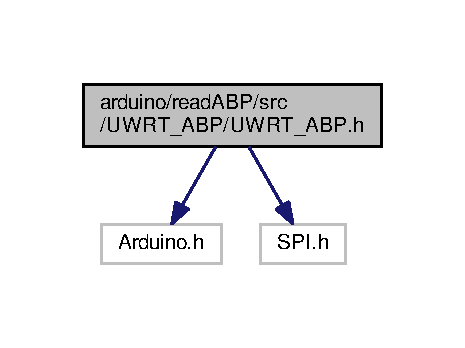
\includegraphics[width=223pt]{UWRT__ABP_8h__incl}
\end{center}
\end{figure}
\subsection*{Classes}
\begin{DoxyCompactItemize}
\item 
class \hyperlink{classUWRT_1_1Abp}{U\+W\+R\+T\+::\+Abp}
\begin{DoxyCompactList}\small\item\em A\+BP Differential Pressure Sensor object. \end{DoxyCompactList}\item 
class \hyperlink{classUWRT_1_1AbpArray}{U\+W\+R\+T\+::\+Abp\+Array}
\begin{DoxyCompactList}\small\item\em Array of A\+BP objects. \end{DoxyCompactList}\end{DoxyCompactItemize}
\subsection*{Macros}
\begin{DoxyCompactItemize}
\item 
\#define \hyperlink{UWRT__ABP_8h_adc6568b52529df9d20dd786cc39c7a67}{P\+\_\+\+M\+IN}~-\/1.\+0f\hypertarget{UWRT__ABP_8h_adc6568b52529df9d20dd786cc39c7a67}{}\label{UWRT__ABP_8h_adc6568b52529df9d20dd786cc39c7a67}

\begin{DoxyCompactList}\small\item\em Minimum pressure for the A\+BP sensor in psi. \end{DoxyCompactList}\item 
\#define \hyperlink{UWRT__ABP_8h_a86355cc297e2a38312a982605ab7b96c}{P\+\_\+\+B\+\_\+\+S\+L\+O\+PE}~0.\+00015259f\hypertarget{UWRT__ABP_8h_a86355cc297e2a38312a982605ab7b96c}{}\label{UWRT__ABP_8h_a86355cc297e2a38312a982605ab7b96c}

\begin{DoxyCompactList}\small\item\em Pressure (psi) per count. \end{DoxyCompactList}\item 
\#define \hyperlink{UWRT__ABP_8h_a862b69b3e056a479017ebd4068d88d94}{O\+\_\+\+M\+IN}~1638\hypertarget{UWRT__ABP_8h_a862b69b3e056a479017ebd4068d88d94}{}\label{UWRT__ABP_8h_a862b69b3e056a479017ebd4068d88d94}

\begin{DoxyCompactList}\small\item\em Minimum output (counts) \end{DoxyCompactList}\item 
\#define \hyperlink{UWRT__ABP_8h_af83877dd89769b83f81b4b7d019e7039}{S\+P\+I\+\_\+\+B\+A\+UD}~800000\hypertarget{UWRT__ABP_8h_af83877dd89769b83f81b4b7d019e7039}{}\label{UWRT__ABP_8h_af83877dd89769b83f81b4b7d019e7039}

\begin{DoxyCompactList}\small\item\em Baudrate to use for S\+PI. \end{DoxyCompactList}\end{DoxyCompactItemize}


\subsection{Detailed Description}
Class definitions for S\+PI communications with Honeywell A\+BP Differential Pressure Sensors on Arduino. 

\begin{DoxyAuthor}{Author}
Benji Justice (\href{mailto:justice.251@osu.edu}{\tt justice.\+251@osu.\+edu}) 
\end{DoxyAuthor}
\begin{DoxyVersion}{Version}
0.\+1 
\end{DoxyVersion}
\begin{DoxyDate}{Date}
2019-\/02-\/03
\end{DoxyDate}
\begin{DoxyCopyright}{Copyright}
Copyright (c) 2019 
\end{DoxyCopyright}

%--- End generated contents ---

% Index
\backmatter
\newpage
\phantomsection
\clearemptydoublepage
\addcontentsline{toc}{chapter}{Index}
\printindex

\end{document}
